%! Author = Filippo Vissani
%! Date = 08/02/24
% !TeX root = ../thesis-main.tex

%----------------------------------------------------------------------------------------
\chapter{Evaluation}
\label{chap:evaluation}
%----------------------------------------------------------------------------------------

\section{Testing}

\section{Analysis of the Ergonomics of the Proposed Models}

\begin{figure}
    \centering
    \begin{subfigure}[b]{.15\textwidth}
        \centering
        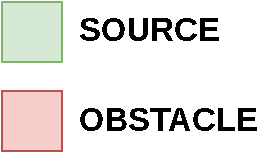
\includegraphics[width=\textwidth]{figures/gradient-environment-legend.pdf}
        \label{fig:gradient-legend}
    \end{subfigure}
    \hfill
    \begin{subfigure}[b]{.49\textwidth}
        \centering
        
\includegraphics[width=\textwidth]{figures/palette-cropped2.png}
        \label{fig:gradient-palette}
    \end{subfigure}
    \hfill
    \begin{subfigure}[b]{.49\textwidth}
        \centering
        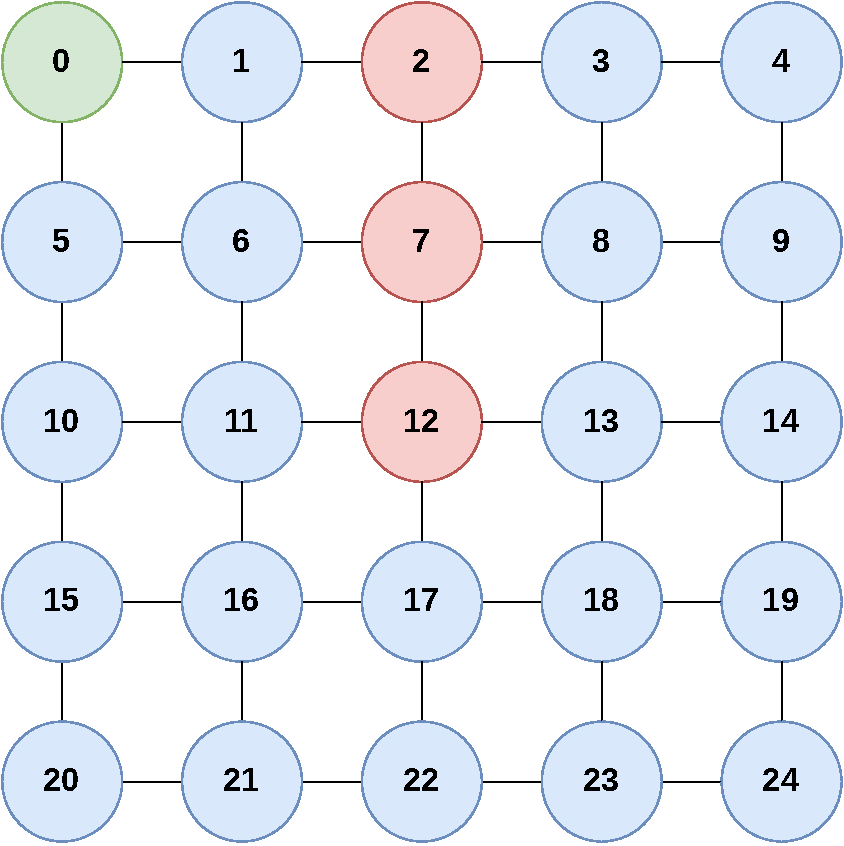
\includegraphics[width=\textwidth]{figures/gradient-environment.pdf}
        \caption{TODO.}
        \label{fig:gradient-envronment}
    \end{subfigure}
    \hfill
    \begin{subfigure}[b]{.49\textwidth}
        \centering
        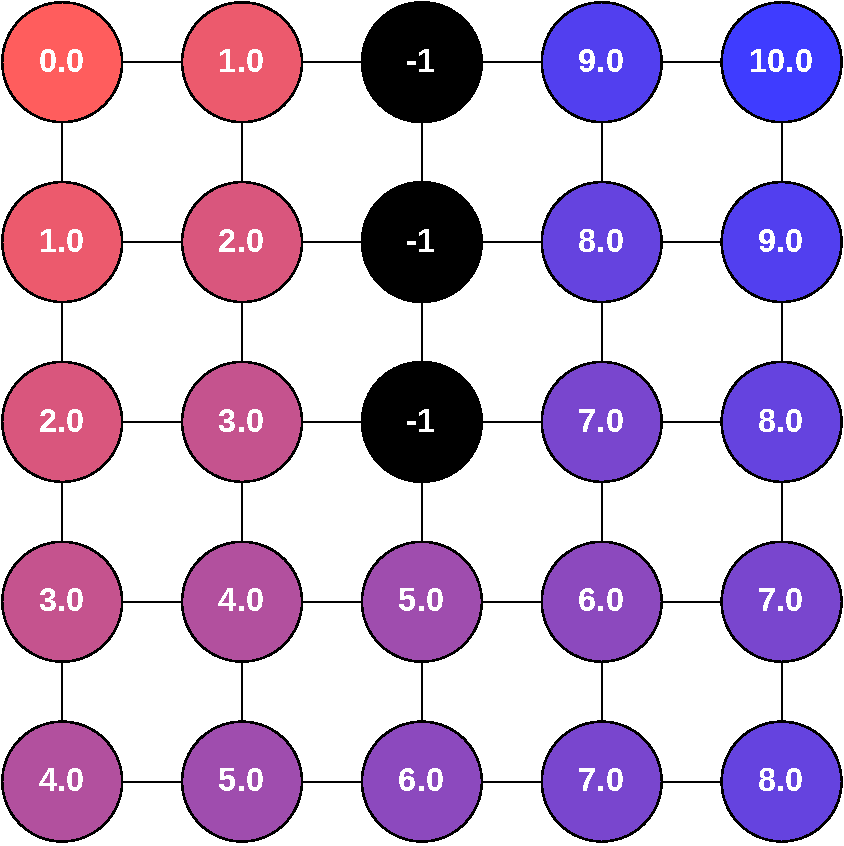
\includegraphics[width=\textwidth]{figures/gradient-environment-execution.pdf}
        \caption{TODO.}
        \label{fig:gradient-envronment-execution}
    \end{subfigure}
\end{figure}

\lstinputlisting[float,language=kotlin,label={lst:simulation-configuration},caption=TODO.]{listings/simulation-configuration.kt}

\subsection{Purely Reactive Model}

\lstinputlisting[float,language=kotlin,label={lst:gradient-obstacles-prm},caption=TODO.]{listings/gradient-obstacles-prm.kt}

\subsection{Model with Reactive Messages and Sensors}

\lstinputlisting[float,language=kotlin,label={lst:gradient-obstacles-rmsm},caption=TODO.]{listings/gradient-obstacles-rmsm.kt}
